\chapter{Implementation} \label{chapter:implementation}
In this chapter, we describe the implementation of the proposed design changes and the technologies used.

\section{Software Stack}

The proposed design involves many parts that we had to extend:
\begin{itemize}
      \tightlist
      \item Kubernetes Scheduler, written in Go.
      \item Kubernetes Cluster Autoscaler, written in Go.
      \item Rok CSI driver, written in Python.
\end{itemize}

It also introduces a new component, the Rok Scheduler webhook, which we wrote in
Go.

We build the components in a reproducible manner, using Docker containers for
the target language of each component. To describe and automate the build
process, we used Dockerfiles and Makefiles.

In order to deploy the components (Cluster Autoscaler, Rok Scheduler, Rok
Scheduler webhook) on the cluster, we write YAML manifests that use the
declarative API of Kubernetes to describe the necessary resources. To ease out
the manifests management, we use the \textit{Kustomize} tool. Kustomize is a
configuration management solution that leverages layering to preserve the base
settings of the applications and components by overlaying declarative YAML
artifacts (called patches) that selectively override default settings without
changing the original files.


\section{Extending the Rok CSI driver}

In order to extend the Rok CSI driver's node component with the capacity
reporting functionality, we introduce a new thread that periodically calculates
the capacity and updates the capacity on the \co{Node} object on the API Server. The
Python thread issues commands to the underlying Logical Volume Manager to fetch
the Rok VG size. We introduce an argument {\co{--capacity-poll-interval}} to
configure how long the thread waits before updating the storage capacity.


\lstinputlisting[label={listing:rok-capacity},language=Python,caption={The thread of Rok CSI driver that updates the available capacity}]{code/rok-capacity.python}

\section{Extending the Kubernetes Scheduler}

The VolumeBinding plugin of the Kubernetes Scheduler imports and uses the
\texttt{scheduling} package located at
\texttt{pkg/controller/volume/scheduling/scheduler\_binder.go}, in the
Kubernetes repo \footnote{\url{https://github.com/kubernetes/kubernetes}}. We
extend the package as follows:

\begin{itemize}
      \tightlist
      \item Introduce a \texttt{hasRokEnoughCapacity(claims\
            {[}{]}*v1.PersistentVolumeClaim,\ node\ *v1.Node)} method, which
            checks if there is enough capacity on the given \texttt{node} to
            provision all the specified Rok PVCs (\texttt{claims}). This method
            executes the following steps:
            \begin{enumerate}
                  \tightlist
                  \item Iterate through the given \co{claims}, and sum their
                        storage requests in
                        \texttt{totalRequestedCapacity}
                  \item Check if the given node has
                        \texttt{rok.arrikto.com/capacity} annotation.
                  \item If the annotation does not exist, or if it exists but is
                        not a valid int, returns \co{false}, which indicates the
                        PVCs can not be provisioned on the examined node.
                  \item If the annotation exists, fetch its value as
                        \texttt{nodeCapacityInBytes}.
                  \item If \texttt{totalRequestedCapacity} $\leq$
                        \texttt{nodeCapacityInBytes} return true, otherwise
                        false.
            \end{enumerate}
            The implementation of the method is exposed in listing
            \ref{listing:hasrokenough}.
      \item Extend the \texttt{checkVolumeProvisions()} method of the
            \co{VolumeBinding} plugin to gather all the Rok PVCs, (PVCs
            provisioned by \texttt{rok.arrikto.com}), and pass them to
            \texttt{hasRokEnoughCapacity()}, in order to check if there is
            enough capacity for all of them to be provisioned on a selected
            node. The implementation is show at Listing
            \ref{listing:checkvolumeprovisions}.
      \item Treat the case that the \texttt{rok.arrikto.com/capacity} does not
            exist as \texttt{zero} capacity, i.e., the volumes can not be
            provisioned.
\end{itemize}

\lstinputlisting[label={listing:hasrokenough},language=Golang,caption={Implementation of the hasRokEnoughCapacity() method}]{code/scheduler-rok-has-enough.go}
\lstinputlisting[label={listing:checkvolumeprovisions},language=Golang,caption={Extension of the checkVolumeProvisions() method}]{code/scheduler-volume-binding.go}

We compile the Rok Scheduler and build its Docker image using the Makefile the
upstream project provides. We use YAML manifests and the Kustomize tool to
deploy the Rok Scheduler as a \co{Deployment} along with any other RBAC
resources it needs for its operation.

\section{Implementing the Rok Scheduler Webhook}

We implement the Rok Scheduler webhook that will mutate the Pods to use the Rok
Scheduler, in a manner it can be reused and easily configured. 

We expose the following configuration options:
\begin{itemize}
      \item {\co{--annotation-optout}}:  Annotation key that if present
            on the Pod, the Pod will not be mutated. The default value is
            \co{arrikto.com/skip-rok-scheduler-webhook}. This parameters allows
            the user to skip the mutation of a Pod in the webhook server, even
            though the API server admitted that Pod for mutation. We will refer
            to it as the ``\textit{opt-out annotation}''.
      \item {\co{--namespaces-optin}}: A comma-separated list of
            namespaces or namespaces globs. If a Pod matches against one of
            these namespaces it will get mutated. The default value is
            \co{``*''}, which matches against all namespaces. We will refer to
            it as the ``\textit{opt-in namespaces}''.
      \item {\co{--scheduler-name}}: The name of the scheduler that will
            be set on the Pod. The default  value is \co{rok-scheduler}.
\end{itemize}
For a complete list of arguments, see the \co{main()} method of the webhook in
Listing \ref{listing:webhook-main}.

The \co{Handle()} method of the webhook handles a single admission request as
follows:
\begin{enumerate}
      \tightlist
      \item If the Pod it has the opt-out annotation, do not mutate it.
      \item Check the namespace of the Pod against each namespace glob. If
            the namespace does not match any glob, do not mutate it.
      \item In all other cases, mutate the Pod by adding the scheduler name on
            its \\ \co{spec.SchedulerName} field.
\end{enumerate}

For the full implementation of the method, see Listing
\ref{listing:webhook-handle}.

We implement the Rok Scheduler Webhook using the \co{webhook} package of the
controller-runtime library of Go. The Kubernetes controller-runtime is a set of
go libraries for building controllers. For implementing the glob functionality
of the \co{--namespaces-optin} flag, we used the \co{glob} module of Go. 

Finally, in order for the Pods to be admitted and sent to the webhook, we
instruct the API Server to do so by creating a \co{MutatingWebhookConfiguration}
object (see Listing \ref{listing:webhook-object}). The
MutatingWebhookConfiguration we specify admits any newly created Pods in
namespaces that match the specific namespace selector. The namespace selector
matches against any namespaces that have the label \co{control‐plane: kubeflow}.
We chose to admit Pods only in this namespace since the workload we want to
admit is created in that namespace, but of course, the Pods in any other
namespace can be admitted. The MutatingWebhookConfiguration specifies that the
API server contacts the webhook server at the \co{/mutate} endpoint. It also
specifies a \co{Fail} failure policy so that if the webhook crashes or stops
responding, the creation of new Pods will fail. That is important to ensure
every single Pod is admitted and mutated with the scheduler name.

\lstinputlisting[label={listing:webhook-main},language=Golang,caption={The main() method of the Rok Scheduler Webhook}]{code/mutating-webhook-main.go}
\lstinputlisting[label={listing:webhook-handle},language=Golang,caption={The Handle() method the Rok Scheduler Webhook}]{code/webhook.go}
\lstinputlisting[label={listing:webhook-object},language=yaml,caption={The Rok Scheduler's MutatingWebhookConfiguration}]{code/mutating-webhook.yaml}

To build the Rok Scheduler Webhook and its Docker image, we create a Dockerfile
that instructs the docker to build the binary inside a container that has the
required \texttt{Golang} dependencies. 

We deploy the Rok Scheduler and the Rok Scheduler as \co{Deployment} resources
(see \ref{section:deployment}). The manifests also specify other necessary
resources, such as Roles, RoleBindings, ServiceAccounts, ConfigMaps.

\section{Extending the Cluster Autoscaler}

\subsection{Scale-Down: Rok Volumes Can Be Migrated}
\label{section:implementation-migration}
As explained in the design proposal (see
\ref{section:design-autoscaler-unpinned}), we extend the Cluster Autoscaler to
treat the local volumes of the Rok Storage class as unpinned, i.e., as if they
have no affinities, when evaluating a possible scale-down. In all other cases,
the local volumes shall be evaluated as is, pinned, i.e., having their existing
node affinities. 

To implement the design, we extend the CheckPredicates interface's method with
an extra boolean argument, called \co{simulateUnpinnedVolumes}. We pass down
information from the PredicateChecker methods to the VolumeBinding plugin's
\co{checkBoundClaims()} method. The SchedulerBasedPredicateChecker creates a
\co{cycleState} (see section \ref{section:cycle-state} struct that the plugins
it runs can use for storing data. We extend the \co{cycleState}  with the same
boolean \co{simulateUnpinnedVolumes} field to pass down to the VolumeBinding
plugin information. The full flow of the information whether to simulate
unpinned volumes or not is illustrated in Figure ~\ref{fig:flow-simulate}.

\begin{figure}[ht]
      \centering
      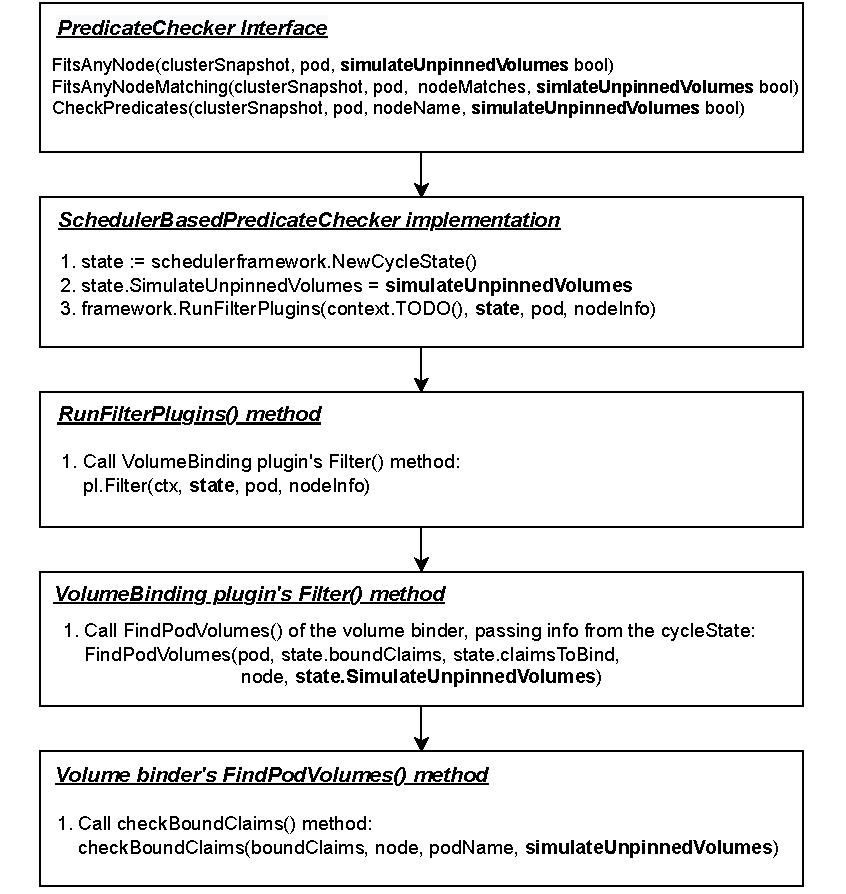
\includegraphics[width=0.8\textwidth]{resources/simulate-unpinned-flow.pdf}
      \caption{The flow of simulateUnpinnedVolumes information}
      \label{fig:flow-simulate}
\end{figure}


We extend the \co{checkBoundClaims()} method, so that if the Rok volumes are
simulated as unpinned (\co{simulateUnpinnedVolumes} is set to \co{true}), it
gathers all the Rok local volumes, and appends them to \co{claimsToProvision},
i.e, it treats them as if they were unbound volumes, in order to check if there
is enough capacity (see (\co{checkVolumeProvision()}) for the volumes to be
provisioned on the examined node. Of course, this approach only checks if the
Rok volumes of a Pod alone can be moved to a different node; it does not ensure
that all the Pods of the node can fit on a different node with regards to their
local storage requests. Listing \ref{listing:check-bound-claims} presents the
code lines that extend the functionality of \co{checkBoundClaims}.

\lstinputlisting[language=Golang,label={listing:check-bound-claims},caption={Extending the logic of checkBoundClaims() when volumes are simulated as unpinned}]{code/find-pod-volumes.go}


\subsection{Scale-Down: Coordinate With the Rok CSI Guard Mechanism}


To implement the design proposal (see section
\ref{section:design-autoscaler-guards}) we implement the following changes,
according to the proposed design:
\begin{itemize}
      \tightlist
      \item Extend the \co{findPlaceFor()} method to ignore the Rok CSI
            Guard Pods and not try to find a place for them on a different node.
      \item Extend the \co{checkPdbs()} method to not check the PodDisruptionBudgets
            of the Rok CSI Guard Pods.
      \item We introduce a flag \co{--max-pod-eviction-time}  so that the
      cluster admins can configure the maximum time Autoscaler tries to evict a Pod
      before giving up.
\end{itemize}

\lstinputlisting[language=Golang,label={listing:ignore-guard},caption={Ignore Rok CSI Guard Pods and their PDBs in scale-down evaluation}]{code/find-place-for.go}

%TODO: code snippet flag


\subsection{Scale-Down: Consider Storage Capacity}
We already covered in section \ref{section:implementation-migration} how we
extended the Autoscaler to simulate the Rok volumes as unpinned when scaling
down and also check if there is enough capacity for each Pod on a different
node.

We also extend the Autoscaler to calculate storage utilization and take it into
consideration when scaling down, by introducing a new flag
``--scale-down-rok-storage-utilization-threshold'' flag with default value
``0.5'' and a \co{CalculateUtilizationOfRokStorage()} method. This method
fetches the values from the capacity annotation and the max capacity label of
the \co{Node} object and calculates the storage utilization. Moreover, we extend
the \co{checkNodeUtilization()} method of the Autoscaler to mark any nodes that
have storage utilization over the storage threshold as unremovable. The
implementation can is shown in Listings \ref{listing:storage-util} and
\ref{listing:node-utilization}.

\lstinputlisting[label={listing:storage-util},language=Golang,caption={Calculate Rok storage utilization}]{code/rok-utilization.go}
\lstinputlisting[label={listing:node-utilization},language=Golang,caption={Mark nodes with high Rok storage utilization as unremovable}]{code/rok-utilization-threshold.go}


\subsection{Scale-Down: Do Not Remove Unready Nodes}

To implement the proposed design and configure the Autoscaler to not removed
unready nodes, we extend the \texttt{--scale-down-unready-time} of the
Autoscaler to accept negative values; if a negative value is provided, then the
scale-down of unready nodes will be disabled.

\subsection{Scale-Up: Consider Storage Capacity}

\paragraph*{Pass the max capacity information to the template}
To implement the scale-up design, we introduce a method
\co{sanitizeRokStorageAnnotations()} that copies the value of the max capacity
label of the \texttt{Node} object to its capacity annotation. If the label does
not exist, it set the capacity annotation to the max 64 bit number.We extend the
\co{sanitizeTemplateNode()} method to call \co{sanitizeRokStorageAnnotations} as
part of the sanitization process.

The implementation of this functionality is shown in Listings
\ref{listing:sanitize-rok} and \ref{listing:sanitize}.

\lstinputlisting[language=Golang,label={listing:sanitize-rok},caption={sanitizeRokStorageAnnotations() method}]{code/scale-up-capacity-label.go}
\lstinputlisting[language=Golang,label={listing:sanitize},caption={Extend sanitizeTemplateNode() to sanitize the Rok storage annotations}]{code/note-template-capacity.go}

\paragraph*{Wait for Rok CSI to run}

We implement this design change by introducing a
\co{FilterOutNodesWithUnreadyCSI()} method to check if a node has the capacity
annotation set. If not, it is implied that the Rok CSI driver is not running on
the node, and it replaces the node with an unready copy. We extend the
\co{obtainNodeLists()} method, to call the \co{FilterOutNodesWithUnreadyCSI}.

Listings \ref{listing:unready-csi} and \ref{listing:unready-csi-obtain} present
the code lines that implement this functionality.

\lstinputlisting[label={listing:unready-csi},language=Golang,caption={FilterOutNodesWithUnreadyCSI() method}]{code/unready-csi.go}
\lstinputlisting[label={listing:unready-csi-obtain},language=Golang,caption={Extend ObtainNodesLit() method to return nodes with unready Rok CSI}]{code/obtain-nodes-list.go}
